\documentclass[12pt,a4paper]{article}
\usepackage[utf8]{inputenc}
\usepackage[english]{babel}
\usepackage[T1]{fontenc}
\usepackage{amsmath}
\usepackage{amsfonts}
\usepackage{amssymb}
\usepackage{graphicx}
\usepackage{titlesec}
\usepackage[left=2cm,right=2cm,top=2cm,bottom=2cm]{geometry}
\usepackage{indentfirst}
\usepackage{listings}
\usepackage{color}
\usepackage{url}
\usepackage{array}

%Pravidlo pro řádkování
\renewcommand{\baselinestretch}{1.5}

%Pravidlo pro začínání kapitol na novém řádku
\let\oldsection\section
\renewcommand\section{\clearpage\oldsection}

%Formáty písem pro nadpisy (-změněno na bezpatkové \sffamily z původního \normalfont
\titleformat{\section}
{\sffamily\Large\bfseries}{\thesection}{1em}{}
\titleformat{\subsection}
{\sffamily\large\bfseries}{\thesubsection}{1em}{}
\titleformat{\subsubsection}
{\sffamily\normalsize\bfseries}{\thesubsubsection}{1em}{}

%Nastavení zvýrazňování kódu v \lslisting
\definecolor{mygreen}{rgb}{0,0.6,0}
\definecolor{mygray}{rgb}{0.5,0.5,0.5}
\lstset{commentstyle=\color{mygreen},keywordstyle=\color{blue},numberstyle=\tiny\color{mygray}}

\author{Štěpán Ševčík}

% pravidlo pro c#

\usepackage{color}
\definecolor{bluekeywords}{rgb}{0.13,0.13,1}
\definecolor{greencomments}{rgb}{0,0.5,0}
\definecolor{redstrings}{rgb}{0.9,0,0}

\lstset{language=[Sharp]C,
	showspaces=false,
	showtabs=false,
	breaklines=true,
	showstringspaces=false,
	breakatwhitespace=true,
	escapeinside={(*@}{@*)},
	commentstyle=\color{greencomments},
	keywordstyle=\color{bluekeywords},
	stringstyle=\color{redstrings},
	basicstyle=\ttfamily
}


\begin{document}

%-------------Úvodni strana---------------
\begin{titlepage}


\includegraphics[width=50mm]{img/FAV.jpg}
\\[160 pt]
\centerline{ \Huge \sc KIV/FJP - Formal Languages and Compilers}
\centerline{ \huge \sc Semestral project}
\\[12 pt]
{\large \sc
\centerline{Crest generation from Blazon}
}


{
\vfill 
\parindent=0cm

\begin{center}
\begin{tabular}{|c | c | c |}
	\hline
	\textbf{Name} & \textbf{Student number} & \textbf{E-mail} \\ \hline
	Jan Vampol & A17N0028P & \\ \hline
	Štěpán Ševčík &  A17N0087P & kiwi@students.zcu.cz \\ \hline
	Zdeněk Valeš & A17N0094P & \\ \hline
\end{tabular}
\end{center}
\textbf{Date:} {\large \today\par} %datum
\textbf{Repository:} \url{https://github.com/Thoronir42/heraldry}

}

\end{titlepage}

%------------------Obsah-------------------
%\newpage
%\setcounter{page}{2}
%\setcounter{tocdepth}{3}
%\tableofcontents
%------------------------------------------

%--------------Text dokumentu--------------


\section{Abstract}
In the medieval heraldry, blazon is used to describe war symbols such as a coat of arms or a similar emblems. If understood as a formal language, blazon can be processed and to a certain level automatically compiled and rendered into an appropriate visual or text representation.

\section{Introduction}
During the medieval ages, a need to distinguish armies arose, which was sated by introduction of Blazon, which is a language designed to describe coats of arms and other aspects of armies.

This semestral projects explores this language and attempts to create a process to automatically compile input blazon through internal structure into a graphical representation.

Along the blazon, this project also briefly introduces the various parts of formal process of translation.

\section{Assignment}
The goal of this project is to:
\begin{itemize}
\setlength\itemsep{-0.5em}
\item formalize blazon into a formal language,
\item design grammar,
\item (partially) implement generator functionality allowing rendition of a crest.
\end{itemize}

\subsection{Analysis}
The blazon language is constructed upon a variety of spoken languages, such as English, Scottish, Czech, German, etc...
For this reason, it was chosen to construct the terminal symbols through vocabularies in form of \textit{comma separated values} files which are composed into a \textbf{Vocabulary} structure.
Using this vocabulary, the input text is transformed into a list of tokens using a process called Lexical Analysis.

These tokens represent terminal symbols of a grammar and are used in the Syntactic Analysis to construct an inner structure.
The Syntactic Analysis follows production rules defined in a grammar of given language.

Lastly this structure is interpreted by a renderer into a desired representation, which can be either textual or visual.

\section{Blazon}
The emergence of heraldry as we know it today was linked to the need to distinguish participants quickly and easily in combat \cite{InternationalHeraldry}.
While quick distinction in battle is the primary reason for blazoning, it's also used as a way to display achievements or clan relations.

Blazon accomplishes this using various elements which in matter of speaking are working together as a building kit. The root of a coat of arms is a field, which can be in a simplest case defined by a Tincture, which is either a solid colour, metallic colour or a pattern called fur. The most common Tinctures are depicted on the Figure \ref{tinctures}. The Rule of Tincture prohibits certain colour combinations although in some cases it is broken intentionally.
\begin{figure}[h]
	\centering
	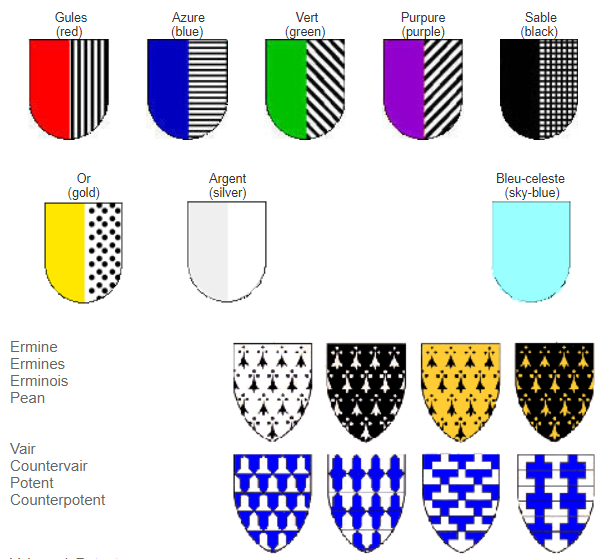
\includegraphics[width=80mm]{img/tinctures.png}
	\caption{Most common tinctures used in blazon \cite{InternationalHeraldry}}
	\label{tinctures}
\end{figure}

In the early days of heraldry, very simple bold rectilinear shapes were painted on shields. These are called ordinaries or sometimes "honourable ordinaries" as they could be easily recognized at a long distance and could be easily remembered.
They therefore served the main purpose of heraldry—identification. \cite{InternationalHeraldry}

\begin{figure}
	\centering
	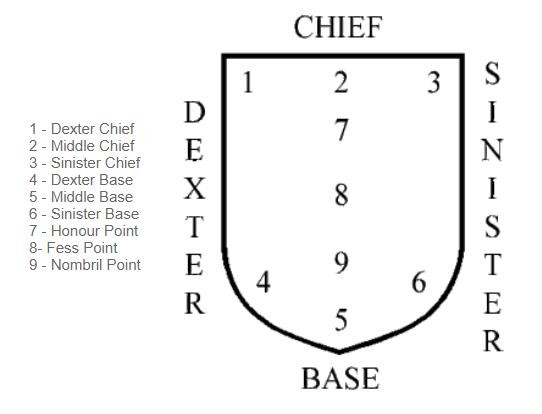
\includegraphics[width=0.5\linewidth]{img/locations}
	\caption{Locations on Coat of Arms}
	\label{fig:locations}
\end{figure}
Any object ranging from simplest shapes to mythical animals can be placed in a field in a role of a Charge.
Sometimes a coat of arms can be introduced as a Charge which usually represents heritage or conjunction of arms and when done so, this inner coat of arms is called inescutcheon.
\pagebreak

Besides placement on a field, charges can be also placed on top of charges or in a one of the locations in chief, on top, or in base, on the bottom, of the shield.
In these locations horizontal alignment can be specified from viewers left to right: Dexter, Middle and Sinister.
These locations and some special points are depicted on Figure \ref{fig:locations}.

Another way of creating more variations is to vary the field. The field can be divided into more than one tincture.
Many coats of arms consist simply of a division of the field into two contrasting tinctures. \cite{InternationalHeraldry}

Few examples of ways to divide the field are split in half vertically "party per pale", split in half horizontally "partly per bend" or split quarterly. These and few more examples are shown on Figure \ref{fig:fielddivisions}.
\begin{figure}[h]
	\centering
	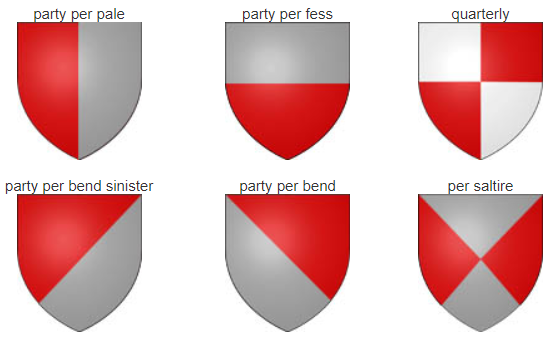
\includegraphics[width=0.60\linewidth]{img/fieldDivisions}
	\caption{Field division examples}
	\label{fig:fielddivisions}
\end{figure}

Portions of field divisions become new fields which are described in same manner as the whole coat of arms in order, unless specified otherwise, from top to bottom, from left to right.

\subsection{Example blazon}
An example of blazoned coat of arms of Slovakia as seen on Figure \ref{fig:slovakia} shows moderately complex coat:
\textit{Gules, a mount of three peaks Azure, issuant therefrom a double cross Argent.}

\begin{figure}
	\centering
	
\includegraphics[width=0.3\linewidth]{img/Slovakia}
	\caption{Coat of arms of Slovakia}
	\label{fig:slovakia}
\end{figure}

In this example, there can be seen a non-typical charge, three-peaked mount, and a double cross comming out of it.

\section{Formal language}
In order to define a formal language, we need to understand the parts it is composed of - the words and the alphabet.
A word (or string) is a finite sequence of items, so-called symbols or letters chosen from a specified finite set called the alphabet.
Examples of common alphabets are e.g. letters in the Latin alphabet (+ interword space, punctuation marks, etc.), and the bits 0 and 1.\cite{ruohonen2009formal}
By definition formal language is a set of words over some alphabet and in other words, formal language is a rule set enumerating possible combinations of words that are.

Current implementation of blazon consists of 15 non-terminal symbols, which are directly rewritten into terminals.

These symbols are:
\begin{itemize}
\setlength\itemsep{-0.5em}
\item \textbf{Tincture (15)} A color or fur-like material,
\item \textbf{Field division(11)} Mean of dividing a field,
\item \textbf{Field variation(9)} Filling pattern definition,
\item \textbf{Division line(9)} Style of dividing line,
\item \textbf{Position(8)},
\item \textbf{Keywords(8)},
\item \textbf{Numbers(20)} 1 through 10 of ordinal and cardinal numbers,
\item \textbf{Ordinaries(18)} Ordinary charges,
\item \textbf{Sub-ordinaries(17)} Subordinary shapes,
\item \textbf{Shape(11)} Shape,
\item \textbf{Shape type(3)} Whether shape is Solid / hollowed,
\item \textbf{Charge properties(5)},
\item \textbf{Charge attitudes(15)},
\item \textbf{Charge attitude directions(3}),
\item \textbf{Charge features(7)}.
\end{itemize}

\newpage
\subsection{Grammar}
Grammar is necessary in order to describe a language and is usually denoted as a quadruple $G = (N, T, S, P)$, where:
\begin{itemize}	\setlength\itemsep{-0.5em}
\item \textbf{N} is a set of non-terminal symbols, which are rewritten into other symbols using production rules,
\item \textbf{T} is a set of terminal symbols, which with few exceptions are never rewritten once defined,
\item \textbf{S} describes the initial symbol of a word,
\item \textbf{P} is a set of production rules.
\end{itemize}

The non-terminal symbols of blazon grammar are listed in previous section and some of these symbols can have subtype technically creating more non-terminal symbols.

The grammar also consists of generic lists which can be made of multiple occurences of any existing symbol separated by \textbf{comma} keywords and the \textbf{and} keyword.

The terminal symbols are loaded into a symbol vocabulary dynamically according to language specified and currently only the old English vocabulary is implemented.

The initial symbol represents the whole coat of arms and the set of production rules is going to be described in section \texttt{Syntactic analysis}.


\section{Compilation}
As previously stated, a language consists of symbols which form words when put together in correct order.

Recognizing and joining these symbols together are first two main disciplines of the compilation whose result is a word or in this case, a blazon instance.
The last stage of compilation is interpretation of a recognized word, which is implemented in form of textual rendition using a vocabulary.


\subsection{Lexical analysis} 
Lexical analysis or tokenization is the first stage of translation process and its role is to recognize language valid symbols.
In this phase the input text is converted into a list of tokens defined by the translator tool.

Most elements of blazon like Tinctures, ordinaries or field divisions are strictly defined and are not likely to change.
Assuming this fact, most of the terminal symbols are listed in a lexical vocabulary and are easily captured into tokens.

Definitions to form tokens are sometimes formed from longer strings of words and mean different things. For this reason, definitions are ordered by length and matched from input text from longest to shortest.
This naive approach covers most of the cases but fails to cover cases in which same word can mean different things in different contexts such as \textit{saltire}, which can either mean a cross or a split tail.

There are some special cases of tokens which would not make sense to parse by a vocabulary, which are:
\begin{itemize}
\setlength\itemsep{-0.5em}
\item Numbers - they are parsed automatically using number rules,
\item Separators, such as dot, comma, colon, etc...,
\item Comments (text in brackets).
\end{itemize}
Each of this case has its custom method of matching from source text but are considerably simple to perform.

On contrary, with exception of simple shapes, it would be practically impossible to list every possible charge.
Because of this, the tokenization is run in two phases: first the vocabulary lookup is run and then the remaining blocks of text are interpreted as Charge tokens.

Each token contains a definition of a recognized element it represents and position in source text which allows description of erroneous token sequences to be projected into source text.

If verbose mode is enabled, lexical analysis also prints the recognized tokens coloured by their types to help understand the text.


\subsection{Syntactic analysis}
This step verifies that the tokens recognized by Lexical analysis follow the grammar rules and are accepted by the language. During this verification, it also interprets these tokens into structured objects.
Each non-terminal symbol from the grammar can be represented as a state while terminal symbols are the tokens being processed.

Because of the blazon nature of field division rules, the constructed representation resembles a tree with its root being the whole coat of arms, its branches representing field divisions and its leaves describing blazon elements.

The implemented grammar is of type LL(1), which means it allows lookahead of one terminal symbol, although most rules work with only the immediate symbol.
Using this approach it is possible to compile most of targeted cases which will be walked through in the Results section.

The grammar is based on the examples of blazons in old English language and covers most of the important elements such as:
\begin{itemize}
\setlength\itemsep{-0.5em}
\item Single tincture and pattern fillings
\item Custom tincture furs
\item Fields with single charge
\item Charges with tinctured properties
\item Quarterly and Partly per- field divisions
\item Ordinaries overall divided field
\end{itemize}

The production rules are realized by methods of \textit{Compiler} classes in the \textbf{Heraldry.SyntacticAnalysis.Compilers} namespace.
These methods form a structure representing grammar and validate a correct token order. The result of each of these methods is one of the elements forming the internal blazon structure.

An example compile method representing production rule for fur tincture with optional custom tinctures is displayed by Listing \ref{lst:compile-fur-filling}.
\newpage
\begin{lstlisting}[frame=single,label={lst:compile-fur-filling},caption={Compile method representing production rule of fur filling},captionpos=b,basicstyle=\small]
public  FurTincture Fur()
{
  TinctureDefinition definition = PopDefinition<TinctureDefinition>(DefinitionType.Tincture, TinctureType.Fur);
  FurTincture tincture = definition.Tincture as FurTincture;

  if(NextTokenIs(DefinitionType.Tincture))
  {
    tincture.PrimaryColor = NonFurTincture();
    PopTokenAs(DefinitionType.KeyWord, KeyWord.And);
    tincture.SecondaryColor = NonFurTincture();
  }

  return tincture;
}
\end{lstlisting}

\subsection{Semantic analysis} 
An optional step after syntactic analysis comes the Semantic analysis whose role is to verify the structure it built.
This step usually does not affect the compilation process and instead can detect errors of various severities.

For example breach of the rule of the Tincture might mean a soft warning while invalid amount of specified fields in a division is a fatal error.

Current compilation implementation contains hints of semantic analysis within the syntactic analysis elements.

Potential extension of Semantic analysis part is to check for re-definition of charge features which the grammar has no chance of preventing since the features can be defined in any order 

\subsection{Crest rendition}
The last step of the process is rendition and its sole purpose is to interpret the recognized structure into desired format.

While the primary goal of this process was to create a visual representation, this project currently only consist of text rendition due mismatch of the extent of the project and provided manpower.

The text rendition is made possible thanks to the definition structure and uses same vocabulary as the Lexical Analysis.
Using this vocabulary, a definer is created which looks up an appropriate definition and retrieves the character sequence defining requested non-terminal symbol.
If the definer is not able to find desired definition, it returns a fall-back text describing the element which was to be rendered.

Thanks to the nature of blazon, the fields are isolated and do not affect each other and therefore it is possible to traverse through the tree structure, rendering each field individually.

The rendition process follows roughly the same pattern as in which the Syntactic analysis works and even the \textbf{Compiler} class structure is closely reflected by a \textbf{Printer} class structure.

Take a note that the charges are interpreted in this phase and while it was practically impossible to recognize every one of them, rendering any possible charge is even tougher task.
When an unrecognised charge is encountered, the renderer warns about this fact and displays a fall-back charge in its place.

\section{Test cases and results}
The blazon compiler was developed to compile two examples: the Coat of arms of Hugh Despenser the Younger and the Coat of arms of the Czech Republic.\\

The first example, Arms of Hugh Despenser, displayed on Figure \ref{fig:despenser}, blazoned \\
\textit{ Quarterly: 1st and 4th Argent; 2nd and 3rd Gules, a fret or overall a bend sable.}
is fully recognized and rendered by current compilation implementation.

\begin{figure}[h]
	\centering
	
\includegraphics[width=0.2\linewidth]{img/Despenser}
	\caption{Coat of arms of Hugh Despenser}
	\label{fig:despenser}
\end{figure}


The second example, Coat of arms of the Czech Republic is displayed on Figure \ref{fig:czech-large} and blazoned \\
\textit{Quarterly: first and fourth gules, a lion rampant queue forchée argent armed, langued and crowned Or (Bohemia); second azure, an eagle displayed chequé gules and argent armed, langued and crowned Or (Moravia); third Or, an eagle displayed sable armed and langued gules crowned of the field and charged on the breast with a crescent terminating in trefoils at each end with issuing from the centrepoint a cross patée argent (Silesia).}

Current compilation implementation fails to cover reference filling and the charge on Sliesia's eagle breasts as the charge itself is rather complicated and its unconventional placement is technically more difficult to recognize.
In order to recognize the placement, it would be necessary to recognize word types of underlying language.

The blazon, reduced of the crescent and reference filling definition (the \textit{of the field}, as in \textit{the same color as the field}), is properly recognized by implemented grammar and then rendered.

This blazon consists of most of the trivial blazon elements and can serve as a reference to most of the simple blazons.

\begin{figure}[h]
	\centering
	
\includegraphics[width=0.2\linewidth]{img/Czech-large}
	\caption{Coat of arms of the Czech Republic}
	\label{fig:czech-large}
\end{figure}

\newpage
The goal of this project was to create a grammar which would recognize the coat of arms of Churchill, which can be seen on Figure \ref{fig:churchill}.

This arms is blazoned by:\\
\textit{Quarterly 1st and 4th Sable a lion rampant on a canton Argent a cross Gules;
2nd and 3rd quarterly Argent and Gules in the 2nd and 3rd quarters a fret Or overall on a bend Sable three escallops of the first and as an augmentation in chief an inescutcheon, Argent a cross Gules and thereon an inescutcheon Azure, three fleurs-de-lis Or.}

\begin{figure}[h]
	\centering
	
\includegraphics[width=50mm]{img/512px-Arms_of_Winston_Churchill.png}
	\caption{Arms of Churchill rendered \cite{ArmsOfChurchillImg}}
	\label{fig:churchill}
\end{figure}

While it was possible to implement nested quarterly division, the compilation of multiple charges in a field, Ordinary as a field or inescutcheon placement are not parts of currently implemented grammar.

\section{Application usage}
Besides the business logic, the application consists of a command line interface which is used to specify the compilation parameters.
The CLI displays the options if invalid parameters were specified or if the \texttt{--help} option is present in run arguments as seen in \ref{fig:cli-help}.
The parameters of the application is the input file (required) and output file (optional).

In order to run properly, the application needs to be placed along a directory \texttt{resources} containing vocabulary directories.
The language of vocabulary can be specified as one of the options.

The easiest mean of compilation is through Visual Studio IDE, which also provides means of fetching dependencies, running unit tests and debugging the whole project.

\begin{figure}[h]
	\centering
	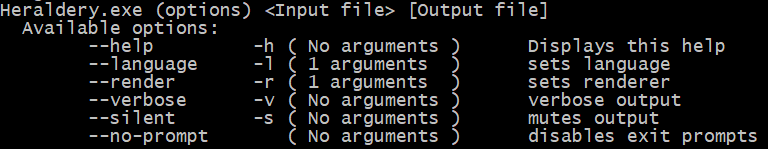
\includegraphics[width=1\linewidth]{img/cli-help}
	\caption{Help output}
	\label{fig:cli-help}
\end{figure}


\section{Conclusion}

We were able to design an extensible grammar which supports most of the simple elements and structures of blazon.

The most difficult tasks were to design the internal structure which went through several iterations of adjustments and to design the compilation process which would fill this structure.
Although we did not manage to fine tune these aspects, they serve their purpose in most of the simpler use cases.

The resulting application demonstrates the possibility to process a language which is human readable and rendition of recognized structure.
While it does not render this structure into graphical format as it was originally planned, implementation of this feature is a question of creating a module respecting a simple interface.

We have tried to keep things separated using the DRY principle, which helped us maintain clean composition and simple functionality verification using unit tests.

\bibliographystyle{abbrv}
{\raggedright\small
	\bibliography{blason}
}

%------------------------------------------



\end{document}
